\tikzset{every picture/.style={line width=0.75pt}} %set default line width to 0.75pt        
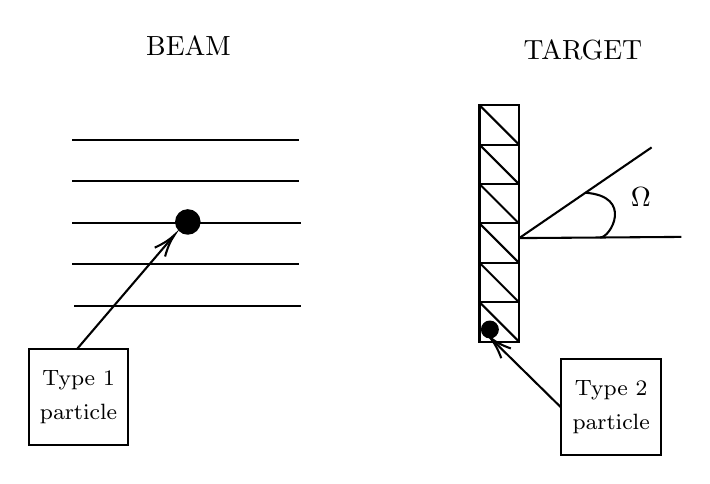
\begin{tikzpicture}[x=0.75pt,y=0.75pt,yscale=-1,xscale=1]
%uncomment if require: \path (0,300); %set diagram left start at 0, and has height of 300
%Straight Lines [id:da7601078847096199] 
\draw    (90,80) -- (199.3,80) ;
%Straight Lines [id:da41431446732450006] 
\draw    (90,100) -- (199.3,100) ;
%Straight Lines [id:da7406610884448859] 
\draw    (90,120) -- (200.3,120) ;
%Straight Lines [id:da5555389414112442] 
\draw    (90,140) -- (199.3,140) ;
%Straight Lines [id:da7113604441316939] 
\draw    (91,160) -- (200.3,160) ;
%Shape: Circle [id:dp6032562484660473] 
\draw  [fill={rgb, 255:red, 0; green, 0; blue, 0 }  ,fill opacity=1 ] (140,119.6) .. controls (140,116.48) and (142.53,113.95) .. (145.65,113.95) .. controls (148.77,113.95) and (151.3,116.48) .. (151.3,119.6) .. controls (151.3,122.72) and (148.77,125.25) .. (145.65,125.25) .. controls (142.53,125.25) and (140,122.72) .. (140,119.6) -- cycle ;
%Straight Lines [id:da4553990376870143] 
\draw    (92.3,180.8) -- (138,127.32) ;
\draw [shift={(139.3,125.8)}, rotate = 490.52] [color={rgb, 255:red, 0; green, 0; blue, 0 }  ][line width=0.75]    (10.93,-3.29) .. controls (6.95,-1.4) and (3.31,-0.3) .. (0,0) .. controls (3.31,0.3) and (6.95,1.4) .. (10.93,3.29)   ;
%Shape: Square [id:dp6385245267322448] 
\draw   (286.2,158.26) -- (305.18,158.26) -- (305.18,177.23) -- (286.2,177.23) -- cycle ;
%Straight Lines [id:da048366194956986464] 
\draw    (286.2,158.26) -- (305.18,177.23) ;
%Shape: Rectangle [id:dp3214112118743824] 
\draw   (286.2,139.28) -- (305.18,139.28) -- (305.18,158.26) -- (286.2,158.26) -- cycle ;
%Straight Lines [id:da08317295232905786] 
\draw    (286.2,139.28) -- (305.18,158.26) ;
%Shape: Square [id:dp9323954113559714] 
\draw   (286.2,120.3) -- (305.18,120.3) -- (305.18,139.28) -- (286.2,139.28) -- cycle ;
%Straight Lines [id:da45254561705281793] 
\draw    (286.2,120.3) -- (305.18,139.28) ;
%Shape: Rectangle [id:dp12155363507098405] 
\draw   (286.2,101.33) -- (305.18,101.33) -- (305.18,120.3) -- (286.2,120.3) -- cycle ;
%Straight Lines [id:da8476758996401002] 
\draw    (286.2,101.33) -- (305.18,120.3) ;
%Shape: Rectangle [id:dp34942394137534416] 
\draw   (286.2,82.35) -- (305.18,82.35) -- (305.18,101.33) -- (286.2,101.33) -- cycle ;
%Straight Lines [id:da38815018499337417] 
\draw    (286.2,82.35) -- (305.18,101.33) ;
%Shape: Ellipse [id:dp6086410383693974] 
\draw  [fill={rgb, 255:red, 0; green, 0; blue, 0 }  ,fill opacity=1 ] (287.37,171.42) .. controls (287.37,169.31) and (289.08,167.6) .. (291.19,167.6) .. controls (293.3,167.6) and (295.01,169.31) .. (295.01,171.42) .. controls (295.01,173.52) and (293.3,175.23) .. (291.19,175.23) .. controls (289.08,175.23) and (287.37,173.52) .. (287.37,171.42) -- cycle ;
%Shape: Rectangle [id:dp006552695566079958] 
\draw   (286.2,63.37) -- (305.18,63.37) -- (305.18,82.35) -- (286.2,82.35) -- cycle ;
%Straight Lines [id:da9936025699051918] 
\draw    (286.2,63.37) -- (305.18,82.35) ;
%Straight Lines [id:da19771769575127984] 
\draw    (325.3,208.8) -- (292.61,176.64) ;
\draw [shift={(291.19,175.23)}, rotate = 404.53999999999996] [color={rgb, 255:red, 0; green, 0; blue, 0 }  ][line width=0.75]    (10.93,-3.29) .. controls (6.95,-1.4) and (3.31,-0.3) .. (0,0) .. controls (3.31,0.3) and (6.95,1.4) .. (10.93,3.29)   ;
%Straight Lines [id:da661445200042976] 
\draw    (305.34,127.38) -- (383.4,126.81) ;
%Straight Lines [id:da0566268996079935] 
\draw    (305.34,127.38) -- (369.12,83.68) ;
%Curve Lines [id:da8769720720143497] 
\draw    (337.23,105.53) .. controls (360.55,107.24) and (349.37,127.1) .. (344.37,127.1) ;
% Text Node
\draw    (69,181) -- (117,181) -- (117,227) -- (69,227) -- cycle  ;
\draw (93,204) node   [align=center] {{{\footnotesize Type 1}}\\{{\footnotesize particle}}};
% Text Node
\draw (146,35) node   [align=center] {{BEAM}};
% Text Node
\draw    (325.62,185.8) -- (373.62,185.8) -- (373.62,231.8) -- (325.62,231.8) -- cycle  ;
\draw (349.62,208.8) node   [align=center] {{{\footnotesize Type 2}}\\{{\footnotesize particle}}};
% Text Node
\draw (363.9,107.39) node    {$\Omega $};
% Text Node
\draw (336,37) node   [align=left] {TARGET};
\end{tikzpicture}